前面几章始终假设炮点与检波器均位于同一位置。现实情况是:炮点与检波器之间水平
间距往往多达3公里,这3公里炮检距已可与许多石油储集层的深度相比了。

炮检距是数据分析中的另一种维数。目前,在野外操作中往往用48道左右的记录道来代
表这个维数,不过,几乎没有人相信有48道就足够了,现在多达1024道的记录系统也正在开
始应用。

炮检距这个维数给反射地震学増添了三个重要问题,第一,它使我们能常规地测定地震
波在岩石中之传播速度,在本书以前两章中均是假设已知这种速度。第二,它可使我们得到
冗余数据:它给出同一量的多次独立观测;因干扰噪音相消干涉,观测结果的叠加为讯号增
强提供了潜在可能性。第三,由于炮检距是非零的,偏移处理就得对付另一种复杂因素了,
这是个缺点,在本章末尾,我们将试图同时处理相互矛盾的三个问题,即,倾角、炮检距和
横向速度变化。

从理论上说,不论在纵波或转换波情形下,全都能把反射系数看作是角度的一个函数,
根据这点,似乎炮检距理应能给我们提供识别岩石的可能性。但是实际情况看来是:即使不
是完全不能观测,至少也是不能可靠地观测的。关于转换波,读者可参阅\ref{sec:1.4}节所进行的充
分讨论,这是一个潜在的具有重大实际应用价值的有意义的研究题目;也可参阅Ostrande
( 1984 )、Tatham与Stoffa(1976
)等人的著作。不过,难以观测的原因以及解决困难的
途径等问题不是本书的讨论内容,只得割爱。本书目的只在于使我们能够有效地姓理常规观
测结果。

\subsection{叠加及现测系统图解}
\label{sec:3.0.1}

首先,将炮点与检波点之间的中点定义为$y$,并定义$h$为炮点与检波点之间的水平炮检距
的二分之一
\begin{subequations}
\begin{equation}
y=\frac{g+s}{2}
\label{eq:ex3.0.1a}
\end{equation}
\begin{equation}
h=\frac{g-s}{2}
\label{eq:ex3.0.1b}
\end{equation}
\label{eq:ex3.0.1}
\end{subequations}
在数学方程中利用二分之一炮检距的原因是为使以后的许多方程能简化和系统化。以而
不以来定义炮检距,就使得正炮检距意味着波是沿着正$x$方向传播。在海上勘探情形下,
这意味着假设船是沿$x$轴的负方向航行的。实际上,船可沿任一路程行进,而且进行勘探
时,炮点可以増多或减少。在某些情况下,令野外观测者的炮点编号数取为负值,你就能说
明事实真相。

野外观测时,数据是限定在$(s,g)$空间内。式\ref{eq:ex3.0.1}代表转换至$(y,h)$空间的
坐标变化,对于解释和数据处理,中心点与炮检距这种坐标系特别有用。由于数据也是旅行
时间$t$的函数,所以完整的数据组是位于某一立体体积内。因为要令人满意地显示这样的体
积太困难了,刃惯上都是作切片显示,各个公司关于切扑的名称稍有不同,下列名称看来是
众所周知和得到公认的:\\
$(y,h=0,t)$  零炮检距剖面 \\
$(y,h=h_{min},t)$  近记录道剖面\\
$(s,g,t=const)$  时间切片\\
$(h,y,t=const)$  时间切片\\
$(y,h=const,t)$  共炮检距剖面\\
$(y,h=h_{max},t)$  远记录道剖面\\
$(y=const,h,t)$  共中心点剖面\\
$(s=const,g,t)$  共炮点道集或野外剖面\\
$(s,g=const,t)$  共检波点道集\\

图\ref{fig:ofs/sg}中为各种名称切片的图式。图\ref{fig:ofs/rick}所示为数据立体体积的三个切片,第一种显示模式是“工程画模式”,
第二种显示模式是侧视立方体的各面,但应注意,尽管数据是显示于立方体的各个表面上,
可切片本身却是取自立方体内部,各个切片彼此的横断交叉均用黑线表示。
\begin{figure}[H]
\centering
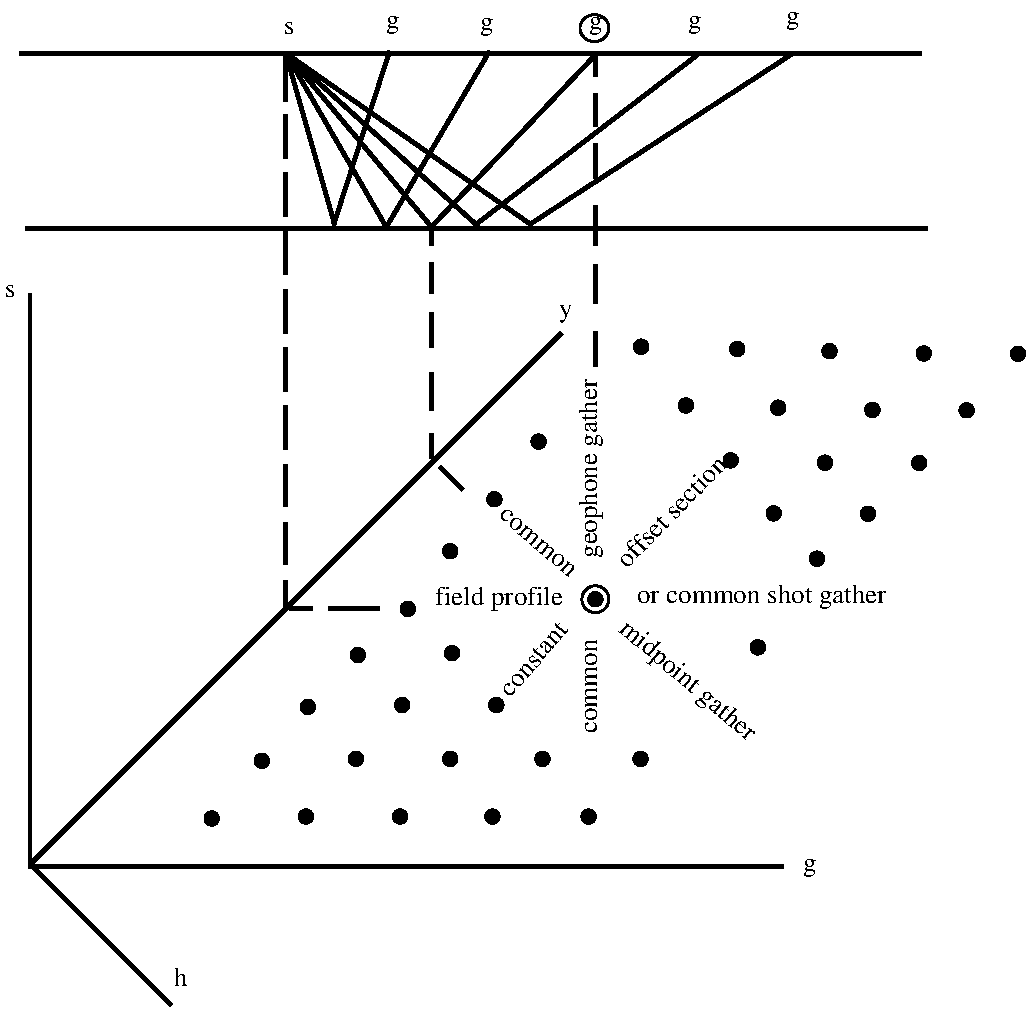
\includegraphics[width=0.65\textwidth]{ofs/sg}
\caption[sg]{顶部图为海上地震记录的野外记录排列,s为炮点,g为检波器。为有助于解释,图中有一水
平反射面。下面的图成为叠加图式(不是透视图)。平面上每个点表示一个可能的地震记录道,可以想象时间
轴是由该平面开始朝向平面之外的。顶部图中的中心检波器(带有圆圈标志者)记录了下图位置上(带圆圈者
)的地震记录道。下图中的各种标记给出了通用的显示名称}
\label{fig:ofs/sg}
\end{figure}

\begin{figure}[H]
\centering
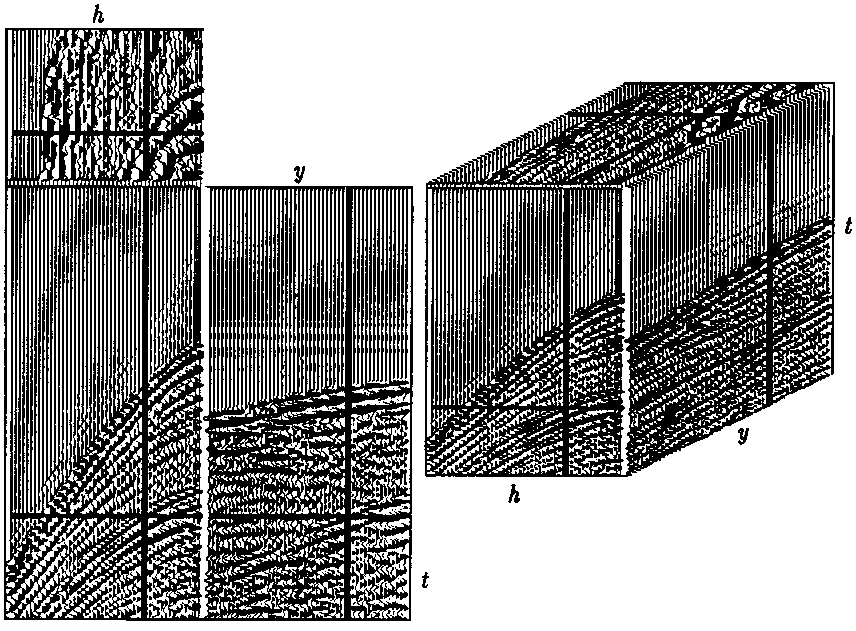
\includegraphics[width=0.65\textwidth]{ofs/rick}
\caption[rick]{Grand Bank地区的数据立方体之各个切片。左图为“工程画”模式,右图取自立方体内之
各切片均表示为立方体上的各侧面}
\label{fig:ofs/rick}
\end{figure}
共深度点(CDP)道集是由工业应用部门定义的,按惯例也可称为共中心点(CMP)
道集。但是在本书中,将对这二者加以区别:共深度点道集(CDP)将被认为是
时间坐标轴按某种速度模型业已拉伸了的共中心点道集(CMP)
\begin{equation*}
(y=const,h,\sqrt{t^2-4h^2/v^2} \quad commom-depth-point\quad gather
\end{equation*}
这种与炮检点有关的拉伸处理使得该道集的时间轴变得更像是深度轴,从而使CDP中的
D是真正与深度有关的。对时间轴进行的这种拉伸处理称作正常时差校正(NMO)。
注意,速度趋于无限大时,拉伸量就趋于零。

在实际应用中,并非按常规把数据显示成炮检距的函数,相反,每个CDP道集都遍及炮
检距求和,求和运算最终得出一个记录道。在每一中心点上可以构制出这样一个记录道,这
些记录道的集合是中心点和时间的函数,称作CDP叠加。粗略地说,CDP叠加剖面像是零
炮检距剖面,不过具有较少干扰的面貌罢了。

构制CDP叠加剖面要求对有利于时差校正的速度迸行选择,这样选择出的速度就称为叠
加速度。叠加速度可以只不过是对地层速度的某些猜涎,再不然用若干个试验速度进行叠
看一看哪个能得出能量最强而噪音最小的CDP叠加结果,因而使速度估计得到改善。在\ref{sec:3.5}
节内将对叠加处理作更多讨论。
